\chapter{MISCELLANEOUS}\label{app:appendix_A}
This chapter discusses how to insert equation, figure and table on \LaTeX~document. All the object in this chapter just the examples to make you ease to write your awesome thesis.
\section{Equation \#examples}
For simple equation, There is a equation $10 + 5x=0$, then determine the value of x by solving that algebraic equation problem. The answer is shown by equation \ref{eq:plus}
	\begin{equation}
		\label{eq:plus}
			\begin{aligned}
			10 + 5x = 0 \\
			5x = -10\\
			x = -2\\
		\end{aligned}
	\end{equation}
Besides that, for complicated equation will be explained as follow. The general equation for a 2D ($N$ by $M$ image) Discrete Cosine Transform is defined by equation \ref{eq:dct}
	\begin{equation}
	\label{eq:dct}
		F(u,v)=\sqrt{\frac{2}{N}} \sqrt{\frac{2}{M}} \sum_{i=0}^{N-1} A(i)*\cos \left(\frac{u(2i+1)\pi}{2N}\right)*\sum_{j=0}^{M-1} A(j)*\cos \left(\frac{v(2j+1)\pi}{2M}\right)*f(i,j)
	\end{equation}
where $A(i)$ is defined as $\left\{ \begin{aligned} \frac{1}{\sqrt{2}}~,~for~u~=~0\\1~,~otherwise \end{aligned} \right.$, while $A(j)$ as $\left\{ \begin{aligned} \frac{1}{\sqrt{2}}~,~for~v~=~0\\1~,~otherwise \end{aligned} \right.$

\section{Figure \#examples}
This section contain how to insert figure (see figure \ref{fig:digital}) and block diagram (see figure \ref{blo:biometrics}). We recommend to use high resolution JPEG or JPG instead PNG format, it will make the compiling process to PDF faster, size of the PDF file is smaller and the quality is image still better when the PDF is print out or zooming out.
	\begin{figure}[H]
		\centering
		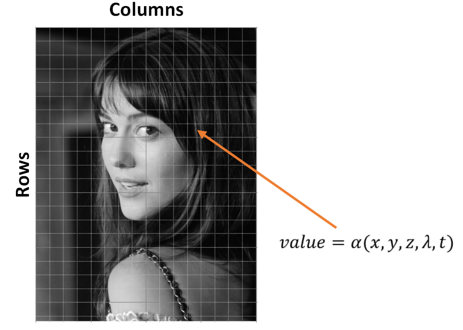
\includegraphics[width=2.5in]{figure/fig_digital}
		\caption{Picture of mary elizabeth winstead}
		\label{fig:digital}
	\end{figure}	


	\begin{figure}[H]
		\centering
		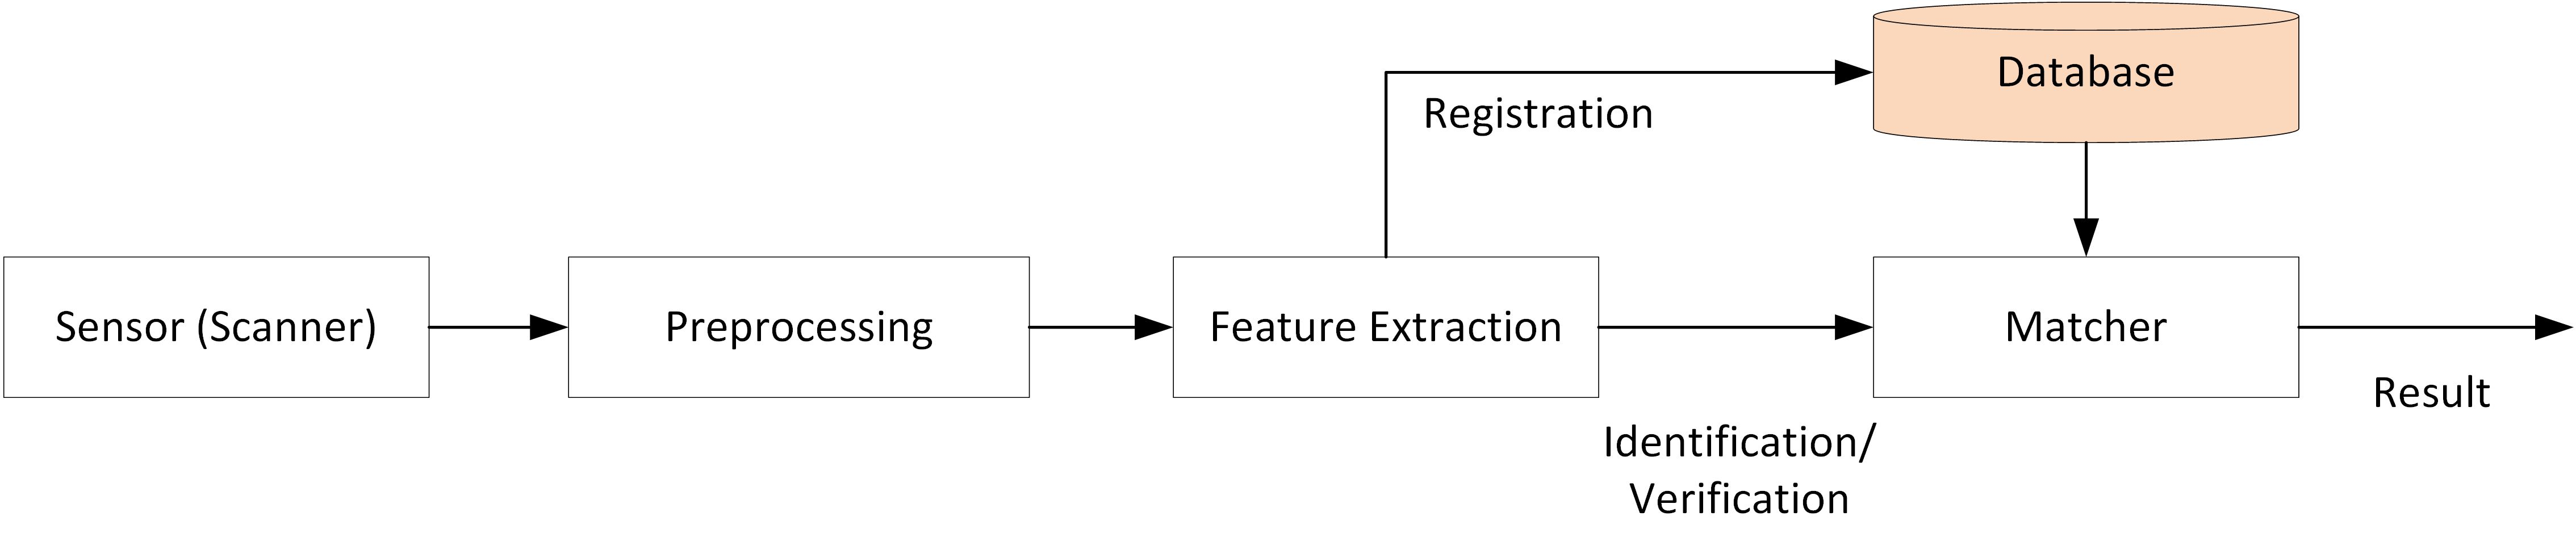
\includegraphics[width=5.5in]{block/gen_biometrics}
		\caption{Example of block diagram.}
		\label{blo:biometrics}
	\end{figure}	
	
\section{Table \#examples}
The regular table (see table \ref{tab:simpleTab}) only can be used in single page. So, for the long table which use multiple pages is recommended to use longtable (see table \ref{tab:fisher_irish})
\begin{enumerate}
	\item Table\\
	Table \ref{tab:simpleTab} will show you how to cite the reference, it can be the author or the year of the reference.
		\begin{table}[H]
		  \centering \caption{Example of Tables}
			\begin{tabular}{|p{1.5cm}|p{3.5cm}|p{3.5cm}|}
			\hline
			\multicolumn{1}{|c|}{\textbf{Reference}} & \multicolumn{2}{c|}{\textbf{Paper or Journal}} \\
			\cline{2-3}    \multicolumn{1}{|c|}{} & \multicolumn{1}{c|}{\textit{\textbf{Authors}}} & \multicolumn{1}{c|}{\textit{\textbf{Full Authors}}} \\
			\hline
			\cite{Jain2007} & \citet{Jain2007}$^a$ & \citefullauthor{Jain2007} \\
			\hline
			\cite{Kong2009} & \citet{Kong2009} & \citefullauthor{Kong2009} \\
			\hline
			\cite{Michael2008} & \citet{Michael2008} & \citefullauthor{Michael2008} \\
			\hline
			\cite{Wang2008} & \citet{Wang2008} & \citefullauthor{Wang2008} \\
			\hline
			\multicolumn{3}{l}{
				\begin{footnotesize}
					$^a$ : \citeyear{Jain2007}.********. 
				\end{footnotesize}
			} \\
			\end{tabular}%
		  \label{tab:simpleTab}%
		\end{table}%
	\item Longtable
		\begin{center}
			\begin{longtable}{|r|r|r|r|r|}\caption{Iris flower data set \#Example of longtable}\label{tab:fisher_irish}\\
				\hline
				\textbf{Sepal length} & \textbf{Sepal width} & \textbf{Petal length} & \textbf{Petal width} & \textbf{Species} \\
				\hline
				\endfirsthead
				\hline
				\textbf{Sepal length} & \textbf{Sepal width} & \textbf{Petal length} & \textbf{Petal width} & \textbf{Species} \\
				\hline
				\endhead
				5.1   & 3.5   & 1.4   & 0.2   & \textit{I. setosa} \\
				\hline
				4.9   & 3     & 1.4   & 0.2   & \textit{I. setosa} \\
				\hline
				4.7   & 3.2   & 1.3   & 0.2   & \textit{I. setosa} \\
				\hline
				4.6   & 3.1   & 1.5   & 0.2   & \textit{I. setosa} \\
				\hline
				5     & 3.6   & 1.4   & 0.2   & \textit{I. setosa} \\
				\hline
				5.4   & 3.9   & 1.7   & 0.4   & \textit{I. setosa} \\
				\hline
				4.6   & 3.4   & 1.4   & 0.3   & \textit{I. setosa} \\
				\hline
				5     & 3.4   & 1.5   & 0.2   & \textit{I. setosa} \\
				\hline
				4.4   & 2.9   & 1.4   & 0.2   & \textit{I. setosa} \\
				\hline
				4.9   & 3.1   & 1.5   & 0.1   & \textit{I. setosa} \\
				\hline
				5.4   & 3.7   & 1.5   & 0.2   & \textit{I. setosa} \\
				\hline
				4.8   & 3.4   & 1.6   & 0.2   & \textit{I. setosa} \\
				\hline
				4.8   & 3     & 1.4   & 0.1   & \textit{I. setosa} \\
				\hline
				4.3   & 3     & 1.1   & 0.1   & \textit{I. setosa} \\
				\hline
				5.8   & 4     & 1.2   & 0.2   & \textit{I. setosa} \\
				\hline
				5.7   & 4.4   & 1.5   & 0.4   & \textit{I. setosa} \\
				\hline
				5.4   & 3.9   & 1.3   & 0.4   & \textit{I. setosa} \\
				\hline
				5.1   & 3.5   & 1.4   & 0.3   & \textit{I. setosa} \\
				\hline
				5.7   & 3.8   & 1.7   & 0.3   & \textit{I. setosa} \\
				\hline
				5.1   & 3.8   & 1.5   & 0.3   & \textit{I. setosa} \\
				\hline
				5.4   & 3.4   & 1.7   & 0.2   & \textit{I. setosa} \\
				\hline
				5.1   & 3.7   & 1.5   & 0.4   & \textit{I. setosa} \\
				\hline
				4.6   & 3.6   & 1     & 0.2   & \textit{I. setosa} \\
				\hline
				5.1   & 3.3   & 1.7   & 0.5   & \textit{I. setosa} \\
				\hline
				4.8   & 3.4   & 1.9   & 0.2   & \textit{I. setosa} \\
				\hline
				5     & 3     & 1.6   & 0.2   & \textit{I. setosa} \\
				\hline
				5     & 3.4   & 1.6   & 0.4   & \textit{I. setosa} \\
				\hline
				5.2   & 3.5   & 1.5   & 0.2   & \textit{I. setosa} \\
				\hline
				5.2   & 3.4   & 1.4   & 0.2   & \textit{I. setosa} \\
				\hline
				4.7   & 3.2   & 1.6   & 0.2   & \textit{I. setosa} \\
				\hline
				4.8   & 3.1   & 1.6   & 0.2   & \textit{I. setosa} \\
				\hline
				5.4   & 3.4   & 1.5   & 0.4   & \textit{I. setosa} \\
				\hline
				5.2   & 4.1   & 1.5   & 0.1   & \textit{I. setosa} \\
				\hline
				5.5   & 4.2   & 1.4   & 0.2   & \textit{I. setosa} \\
				\hline
				4.9   & 3.1   & 1.5   & 0.2   & \textit{I. setosa} \\
				\hline
				5     & 3.2   & 1.2   & 0.2   & \textit{I. setosa} \\
				\hline
				5.5   & 3.5   & 1.3   & 0.2   & \textit{I. setosa} \\
				\hline
				4.9   & 3.6   & 1.4   & 0.1   & \textit{I. setosa} \\
				\hline
				4.4   & 3     & 1.3   & 0.2   & \textit{I. setosa} \\
				\hline
				5.1   & 3.4   & 1.5   & 0.2   & \textit{I. setosa} \\
				\hline
				5     & 3.5   & 1.3   & 0.3   & \textit{I. setosa} \\
				\hline
				4.5   & 2.3   & 1.3   & 0.3   & \textit{I. setosa} \\
				\hline
				4.4   & 3.2   & 1.3   & 0.2   & \textit{I. setosa} \\
				\hline
				5     & 3.5   & 1.6   & 0.6   & \textit{I. setosa} \\
				\hline
				5.1   & 3.8   & 1.9   & 0.4   & \textit{I. setosa} \\
				\hline
				4.8   & 3     & 1.4   & 0.3   & \textit{I. setosa} \\
				\hline
				5.1   & 3.8   & 1.6   & 0.2   & \textit{I. setosa} \\
				\hline
				4.6   & 3.2   & 1.4   & 0.2   & \textit{I. setosa} \\
				\hline
				5.3   & 3.7   & 1.5   & 0.2   & \textit{I. setosa} \\
				\hline
				5     & 3.3   & 1.4   & 0.2   & \textit{I. setosa} \\
				\hline
				7     & 3.2   & 4.7   & 1.4   & \textit{I. versicolor} \\
				\hline
				6.4   & 3.2   & 4.5   & 1.5   & \textit{I. versicolor} \\
				\hline
				6.9   & 3.1   & 4.9   & 1.5   & \textit{I. versicolor} \\
				\hline
				5.5   & 2.3   & 4     & 1.3   & \textit{I. versicolor} \\
				\hline
				6.5   & 2.8   & 4.6   & 1.5   & \textit{I. versicolor} \\
				\hline
				5.7   & 2.8   & 4.5   & 1.3   & \textit{I. versicolor} \\
				\hline
				6.3   & 3.3   & 4.7   & 1.6   & \textit{I. versicolor} \\
				\hline
				4.9   & 2.4   & 3.3   & 1     & \textit{I. versicolor} \\
				\hline
				6.6   & 2.9   & 4.6   & 1.3   & \textit{I. versicolor} \\
				\hline
				5.2   & 2.7   & 3.9   & 1.4   & \textit{I. versicolor} \\
				\hline
				5     & 2     & 3.5   & 1     & \textit{I. versicolor} \\
				\hline
				5.9   & 3     & 4.2   & 1.5   & \textit{I. versicolor} \\
				\hline
				6     & 2.2   & 4     & 1     & \textit{I. versicolor} \\
				\hline
				6.1   & 2.9   & 4.7   & 1.4   & \textit{I. versicolor} \\
				\hline
				5.6   & 2.9   & 3.6   & 1.3   & \textit{I. versicolor} \\
				\hline
				6.7   & 3.1   & 4.4   & 1.4   & \textit{I. versicolor} \\
				\hline
				5.6   & 3     & 4.5   & 1.5   & \textit{I. versicolor} \\
				\hline
				5.8   & 2.7   & 4.1   & 1     & \textit{I. versicolor} \\
				\hline
				6.2   & 2.2   & 4.5   & 1.5   & \textit{I. versicolor} \\
				\hline
				5.6   & 2.5   & 3.9   & 1.1   & \textit{I. versicolor} \\
				\hline
				5.9   & 3.2   & 4.8   & 1.8   & \textit{I. versicolor} \\
				\hline
				6.1   & 2.8   & 4     & 1.3   & \textit{I. versicolor} \\
				\hline
				6.3   & 2.5   & 4.9   & 1.5   & \textit{I. versicolor} \\
				\hline
				6.1   & 2.8   & 4.7   & 1.2   & \textit{I. versicolor} \\
				\hline
				6.4   & 2.9   & 4.3   & 1.3   & \textit{I. versicolor} \\
				\hline
				6.6   & 3     & 4.4   & 1.4   & \textit{I. versicolor} \\
				\hline
				6.8   & 2.8   & 4.8   & 1.4   & \textit{I. versicolor} \\
				\hline
				6.7   & 3     & 5     & 1.7   & \textit{I. versicolor} \\
				\hline
				6     & 2.9   & 4.5   & 1.5   & \textit{I. versicolor} \\
				\hline
				5.7   & 2.6   & 3.5   & 1     & \textit{I. versicolor} \\
				\hline
				5.5   & 2.4   & 3.8   & 1.1   & \textit{I. versicolor} \\
				\hline
				5.5   & 2.4   & 3.7   & 1     & \textit{I. versicolor} \\
				\hline
				5.8   & 2.7   & 3.9   & 1.2   & \textit{I. versicolor} \\
				\hline
				6     & 2.7   & 5.1   & 1.6   & \textit{I. versicolor} \\
				\hline
				5.4   & 3     & 4.5   & 1.5   & \textit{I. versicolor} \\
				\hline
				6     & 3.4   & 4.5   & 1.6   & \textit{I. versicolor} \\
				\hline
				6.7   & 3.1   & 4.7   & 1.5   & \textit{I. versicolor} \\
				\hline
				6.3   & 2.3   & 4.4   & 1.3   & \textit{I. versicolor} \\
				\hline
				5.6   & 3     & 4.1   & 1.3   & \textit{I. versicolor} \\
				\hline
				5.5   & 2.5   & 4     & 1.3   & \textit{I. versicolor} \\
				\hline
				5.5   & 2.6   & 4.4   & 1.2   & \textit{I. versicolor} \\
				\hline
				6.1   & 3     & 4.6   & 1.4   & \textit{I. versicolor} \\
				\hline
				5.8   & 2.6   & 4     & 1.2   & \textit{I. versicolor} \\
				\hline
				5     & 2.3   & 3.3   & 1     & \textit{I. versicolor} \\
				\hline
				5.6   & 2.7   & 4.2   & 1.3   & \textit{I. versicolor} \\
				\hline
				5.7   & 3     & 4.2   & 1.2   & \textit{I. versicolor} \\
				\hline
				5.7   & 2.9   & 4.2   & 1.3   & \textit{I. versicolor} \\
				\hline
				6.2   & 2.9   & 4.3   & 1.3   & \textit{I. versicolor} \\
				\hline
				5.1   & 2.5   & 3     & 1.1   & \textit{I. versicolor} \\
				\hline
				5.7   & 2.8   & 4.1   & 1.3   & \textit{I. versicolor} \\
				\hline
				6.3   & 3.3   & 6     & 2.5   & \textit{I. virginica} \\
				\hline
				5.8   & 2.7   & 5.1   & 1.9   & \textit{I. virginica} \\
				\hline
				7.1   & 3     & 5.9   & 2.1   & \textit{I. virginica} \\
				\hline
				6.3   & 2.9   & 5.6   & 1.8   & \textit{I. virginica} \\
				\hline
				6.5   & 3     & 5.8   & 2.2   & \textit{I. virginica} \\
				\hline
				7.6   & 3     & 6.6   & 2.1   & \textit{I. virginica} \\
				\hline
				4.9   & 2.5   & 4.5   & 1.7   & \textit{I. virginica} \\
				\hline
				7.3   & 2.9   & 6.3   & 1.8   & \textit{I. virginica} \\
				\hline
				6.7   & 2.5   & 5.8   & 1.8   & \textit{I. virginica} \\
				\hline
				7.2   & 3.6   & 6.1   & 2.5   & \textit{I. virginica} \\
				\hline
				6.5   & 3.2   & 5.1   & 2     & \textit{I. virginica} \\
				\hline
				6.4   & 2.7   & 5.3   & 1.9   & \textit{I. virginica} \\
				\hline
				6.8   & 3     & 5.5   & 2.1   & \textit{I. virginica} \\
				\hline
				5.7   & 2.5   & 5     & 2     & \textit{I. virginica} \\
				\hline
				5.8   & 2.8   & 5.1   & 2.4   & \textit{I. virginica} \\
				\hline
				6.4   & 3.2   & 5.3   & 2.3   & \textit{I. virginica} \\
				\hline
				6.5   & 3     & 5.5   & 1.8   & \textit{I. virginica} \\
				\hline
				7.7   & 3.8   & 6.7   & 2.2   & \textit{I. virginica} \\
				\hline
				7.7   & 2.6   & 6.9   & 2.3   & \textit{I. virginica} \\
				\hline
				6     & 2.2   & 5     & 1.5   & \textit{I. virginica} \\
				\hline
				6.9   & 3.2   & 5.7   & 2.3   & \textit{I. virginica} \\
				\hline
				5.6   & 2.8   & 4.9   & 2     & \textit{I. virginica} \\
				\hline
				7.7   & 2.8   & 6.7   & 2     & \textit{I. virginica} \\
				\hline
				6.3   & 2.7   & 4.9   & 1.8   & \textit{I. virginica} \\
				\hline
				6.7   & 3.3   & 5.7   & 2.1   & \textit{I. virginica} \\
				\hline
				7.2   & 3.2   & 6     & 1.8   & \textit{I. virginica} \\
				\hline
				6.2   & 2.8   & 4.8   & 1.8   & \textit{I. virginica} \\
				\hline
				6.1   & 3     & 4.9   & 1.8   & \textit{I. virginica} \\
				\hline
				6.4   & 2.8   & 5.6   & 2.1   & \textit{I. virginica} \\
				\hline
				7.2   & 3     & 5.8   & 1.6   & \textit{I. virginica} \\
				\hline
				7.4   & 2.8   & 6.1   & 1.9   & \textit{I. virginica} \\
				\hline
				7.9   & 3.8   & 6.4   & 2     & \textit{I. virginica} \\
				\hline
				6.4   & 2.8   & 5.6   & 2.2   & \textit{I. virginica} \\
				\hline
				6.3   & 2.8   & 5.1   & 1.5   & \textit{I. virginica} \\
				\hline
				6.1   & 2.6   & 5.6   & 1.4   & \textit{I. virginica} \\
				\hline
				7.7   & 3     & 6.1   & 2.3   & \textit{I. virginica} \\
				\hline
				6.3   & 3.4   & 5.6   & 2.4   & \textit{I. virginica} \\
				\hline
				6.4   & 3.1   & 5.5   & 1.8   & \textit{I. virginica} \\
				\hline
				6     & 3     & 4.8   & 1.8   & \textit{I. virginica} \\
				\hline
				6.9   & 3.1   & 5.4   & 2.1   & \textit{I. virginica} \\
				\hline
				6.7   & 3.1   & 5.6   & 2.4   & \textit{I. virginica} \\
				\hline
				6.9   & 3.1   & 5.1   & 2.3   & \textit{I. virginica} \\
				\hline
				5.8   & 2.7   & 5.1   & 1.9   & \textit{I. virginica} \\
				\hline
				6.8   & 3.2   & 5.9   & 2.3   & \textit{I. virginica} \\
				\hline
				6.7   & 3.3   & 5.7   & 2.5   & \textit{I. virginica} \\
				\hline
				6.7   & 3     & 5.2   & 2.3   & \textit{I. virginica} \\
				\hline
				6.3   & 2.5   & 5     & 1.9   & \textit{I. virginica} \\
				\hline
				6.5   & 3     & 5.2   & 2     & \textit{I. virginica} \\
				\hline
				6.2   & 3.4   & 5.4   & 2.3   & \textit{I. virginica} \\
				\hline
				5.9   & 3     & 5.1   & 1.8   & \textit{I. virginica} \\
				\hline
			\end{longtable}%
		\end{center}%
	\end{enumerate}